\documentclass[t]{sdqbeamer}
%\documentclass[c]{sdqbeamer}

\usepackage{listings}
\usepackage{graphicx}
\usepackage{tabularx}
\usepackage{tikzsymbols}
\usepackage[lined,linesnumbered,ruled,noend]{algorithm2e}

\hypersetup{
	colorlinks=true,
	urlcolor=kit-orange
}

% set sdqbeamer options
\titleimage{blender-render}
\groupname{Algorithm Engineering}
\grouplogo{ae}
\selectlanguage{english}

% define title etc.pp.
\title[SAT Solving]{Practical SAT Solving}
\subtitle{Exercises}
\author{\underline{Ashlin Iser}, Dominik Schreiber}
\date{Mai 5, 2026}

% Existing KIT colors: kit-green, kit-blue, kit-red, kit-gray, kit-orange, kit-lightgreen, kit-brown, kit-purple, kit-cyan
% configure appearance
\setbeamercolor{block title}{bg=kit-blue}
\setbeamercolor{block body}{bg=kit-blue!10}
\setbeamercolor{block title example}{bg=kit-orange}
\setbeamercolor{block body example}{bg=kit-orange!10}
\setbeamertemplate{itemize item}{\color{kit-gray}\textbullet}
\setbeamertemplate{itemize subitem}{\color{kit-gray}\textbullet}
\setbeamercolor{item projected}{bg=kit-gray, fg=kit-gray}
\renewcommand{\insertnavigation}[1]{} % remove navigation bar

% define commands
\input{l00-commands.tex}
\setlength{\itemsep}{1em}

\begin{document}

\begin{frame}
	\thispagestyle{empty}
	\titlepage
\end{frame}

\begin{frame}{Pigeon Hole Principle}
	\vspace{-2em}
	The pigeonhole principle asserts that there is no injective mapping from $m$ pigeons to $n$ holes as long as $m > n$.\\[2em]
	\begin{center}
		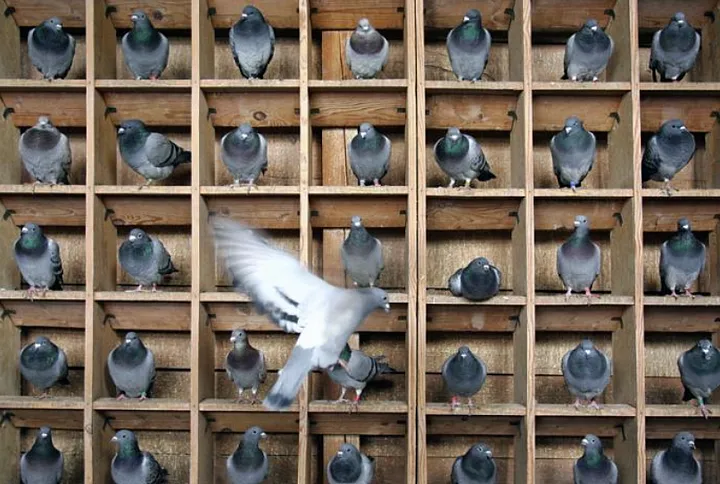
\includegraphics[height=0.6\textheight]{figures/phole.png}~\\[2em]
		\raggedleft {\tiny Image copyright: \url{https://jineralknowledge.com/}}
	\end{center}
\end{frame}

\end{document}
